\chapter{Volume Average Method}
\label{ch:vans}

\section{Introduction}

Maximum 10 lines recalling some of the things said in the previous chapter.

\section{Derivation of VANS equations for 3D incompressible fluids}
%The dynamic of the liquid phase indicated with the subscript $\beta$ is governed by the Navier-Stokes equation for incompressible Newtonian fluid, in presence of a porous medium solid; the equation valid inside the liquid phase are:
%
%\begin{equation}
%\dfrac{\partial \vb}{\partial t} + \vb \cdot \nabla \vb = -\frac{1}{\rho_{\beta}} \nabla \pb + \nub \nabla^2  \vb  + \mathbf{f}, 
%\label{eq:mom}
%\end{equation}
%\begin{equation}
%\nabla \cdot \vb = 0,
%\label{eq:cont}
%\end{equation}
%where $\vb$, $\pb$, $\rho_{\beta}$ and $\nub$ stand, respectively, for  the velocity, the pressure, the density and the kinematic viscosity of the fluid.

\subsection{Definition of the averaging filter}

In the figure \ref{fig:rev} is an illustration of our porous problem; in the same figure we show all the main definition that we need to introduce in order to develop our mathematical approach.


\begin{figure}[h]
	\centering
	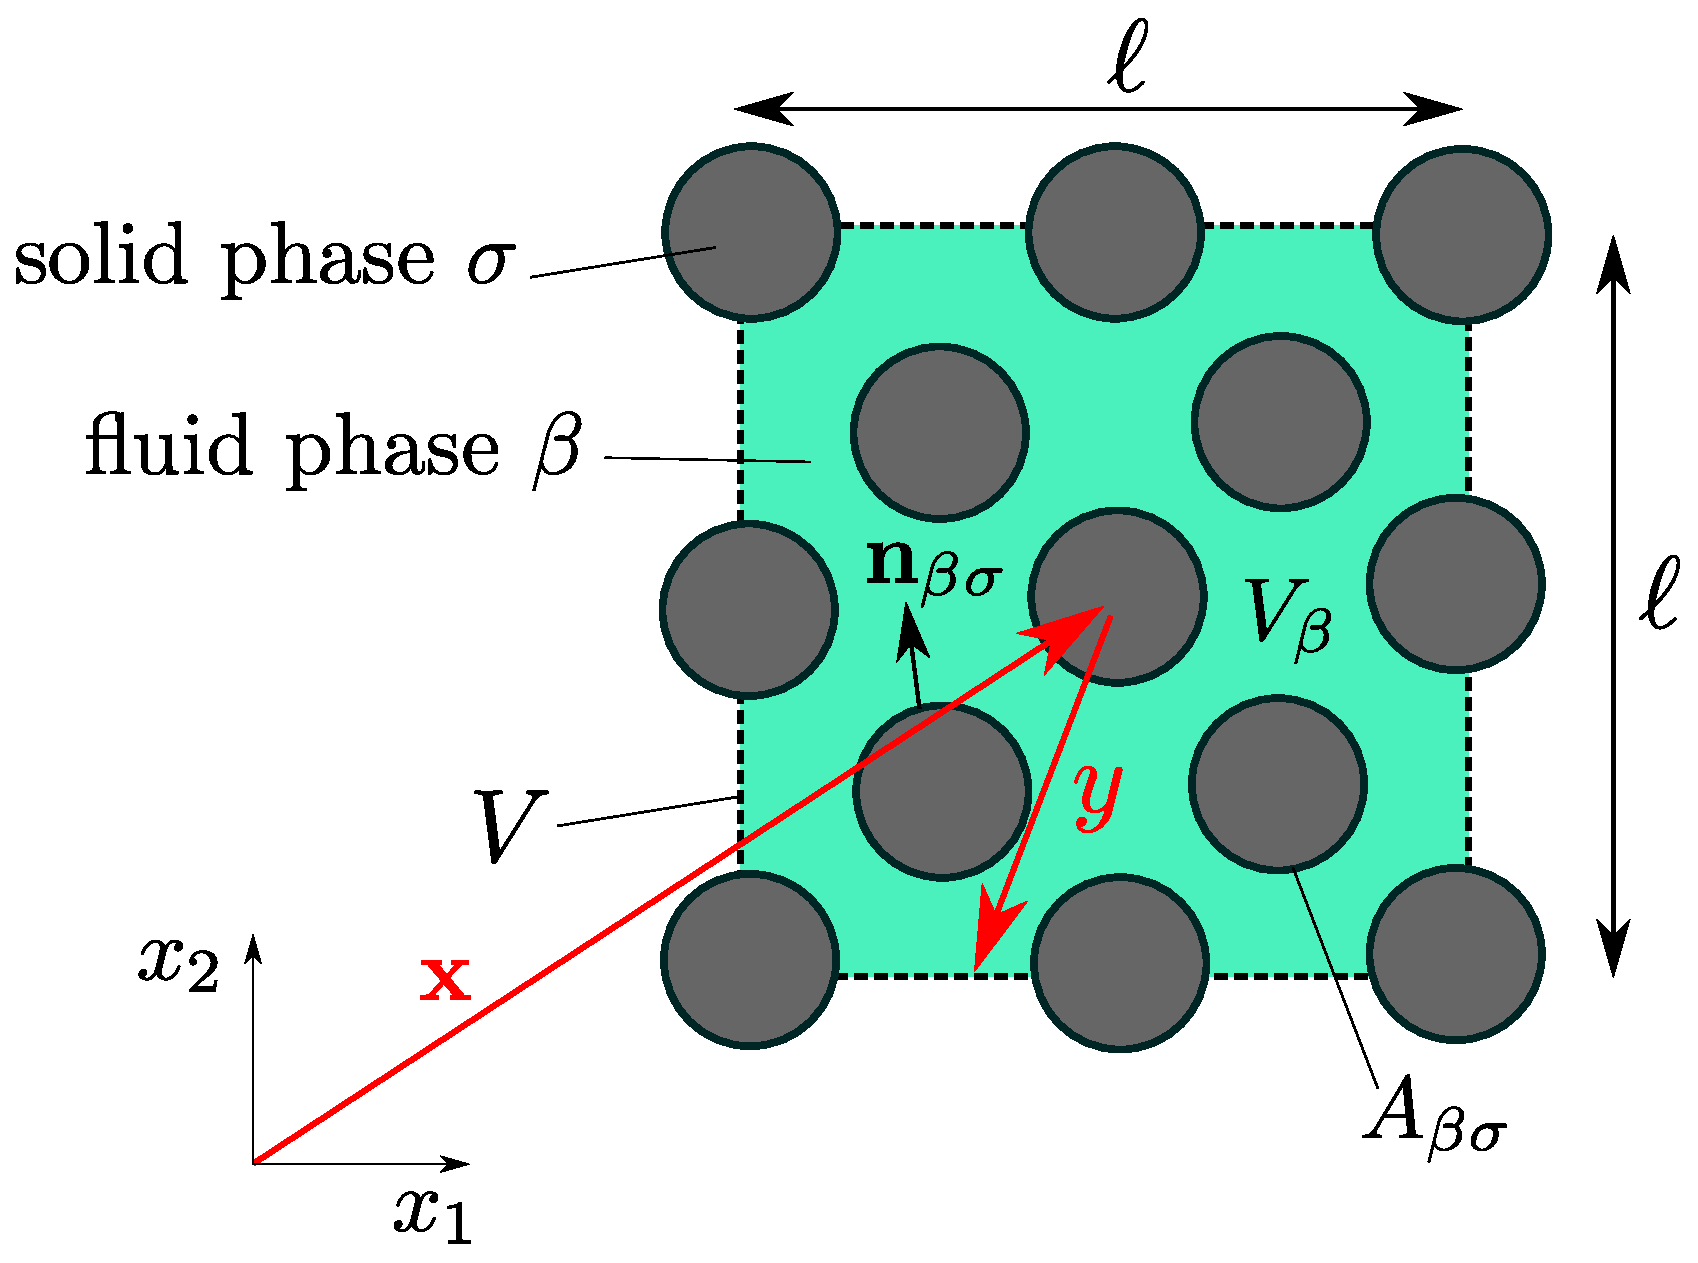
\includegraphics[width=0.7\linewidth]{chapter_2/figure/REV}
	\caption{Illustration of the REV concept.}
	\label{fig:rev}
\end{figure}

Let $\psi_{\beta}$ be an arbitrary vector or scalar field defined on the volume $V$ where $x$ is its centroid, we can define two different spacing average operator.

\begin{equation}
\meani{\psi_{\beta}}|_{\mathbf{x}} = \dfrac{1}{\volb} \int_{\volb(\mathbf{x})}  m(\mathbf{y}) \psi_{\beta}(\mathbf{x}-\mathbf{y}, t) d \, \volb,
\label{eq:avg_intrinsic}
\end{equation}

\begin{equation}
\means{\psi_{\beta}}|_{\mathbf{x}} = \dfrac{1}{V} \int_{\volb} \psi_\beta (\mathbf{x}) d \, \volb,
\label{eq:avg_superficial}
\end{equation}

$\meani{\psi_{\beta}}$ is called the \textit{intrinsic average} and $\means{\psi_{\beta}}$ is the \textit{superficial average}.
The filter $m$ act as a ...
 it is required that
$$
\int_{\volb(\mathbf{x})}  m(\mathbf{y}) d \, \volb = 1
$$

The porosity is defined as:
\begin{equation}
	\varepsilon = \dfrac{\volb}{V}
	\label{eq:porosity}
\end{equation}

So we can defy the relationship:
\begin{equation}
	\means{\psi_{\beta}} =  \varepsilon \meani{\psi_{\beta}}
\end{equation}

\subsection{Theorems involving derivatives of spatial averaging}

\begin{theorem}[Averaging theorem Howes and Withaker, 1985]
\[	\means{\nabla \psi_{\beta}} = \nabla \means{\psi_{\beta}} + \dfrac{1}{V}\int_{A_{\beta \sigma}} \mathbf{n}_{\beta \sigma} \psi_{\beta} dA \]
\end{theorem}


\subsection{Length scale decomposition}

\begin{equation}
	\psi_{\beta} = \meani{\psi_{\beta}} + \tilde{\psi}_{\beta}
 \end{equation}

\subsection{Averaged continuity equations}


\begin{equation}
\nabla \cdot \vb = 0
\label{eq:cont_vans}
\end{equation}

\subsection{Averaged momentum equations}


\begin{equation}
\dfrac{\partial \vb}{\partial t} + \vb \cdot \nabla \vb = -\frac{1}{\rho_{\beta}} \nabla \pb + \nub \nabla^2  \vb  + \mathbf{f}
\label{eq:mom_vans}
\end{equation}



\subsubsection{Interface condition}

Penalization method \citet{angot1999penalization} used in\cite{bruneau2004passive} \cite{bruneau2008numerical} \cite{bruneau2010coupling}...


We think that using a boundary condition at the interface is not a superior approach nor physically neither mathematically.
Using penalization method the slip velocity at the interface can be computed as well as using a boundary condition, and either methods require a parameter to close the formulation, with the advantage using penalization method that the parameter is the spatial distribution of the porosity field that is trivial to compute known the geometry of the medium.

Also in case of very low Reynolds number the boundary condition can be a necessity since the Stokes equations, for the free fluid, and the Darcy one for the porous media are not mathematically compatible; but for $Re>10$ when the Brinkmann model for the porous media is applicable the two set of equations are of the same order and the continuity of pressure and velocity can be imposed directly.

Also there is evidence in literature through numerical and computational experiments \citet{ochoa2017fluid} that exist a transition zone with the size of the pore scale in which the velocity and pressure have a continuous variation.
